\documentclass[11pt, fleqn]{article}

\usepackage[letterpaper, margin=0.7in]{geometry}
\usepackage{graphicx}
\usepackage{subcaption}
\usepackage{cleveref}
\usepackage{listings}
\usepackage{multicol}
\usepackage{tikz}
\usepackage{bm}
\usepackage{minted}
\usetikzlibrary{arrows}
\usepackage{wrapfig}
\usepackage{amsmath}
\usepackage{amssymb}
\usepackage[section]{placeins}
\usepackage{pgfplots,wrapfig}  
\pgfplotsset{compat=newest} 
\pgfplotsset{plot coordinates/math parser=false} 
\newlength\figureheight 
\newlength\figurewidth 
\setlength{\parindent}{0pt}
\newcommand\tab[1][1cm]{\hspace*{#1}}
\usepackage{algorithm}
\usepackage[noend]{algpseudocode}

\let\oldReturn\Return
\renewcommand{\Return}{\State\oldReturn}

\raggedbottom

\begin{document}

\begin{center}

\Large{COMP6212 Assignment 3 : Shakib-Bin Hamid 25250094 sh3g12}

\end{center}

Black-Scholes arrived at a closed form solution of the derivative pricing problem under some strict conditions. Some of these conditions can be eased by creating a binomial lattice based on probabilities on returns. However, these are still parametric methods and sensitive to the underlying stochastic process for $S(t)$, the stock price over time. Misspecification of it will lead to systematic errors in the option's price calculation, i.e. the performance of the parametric models is closely tied with the ability to capture the dynamics of underlying asset or stock.\\

On the other hand, learning networks like RBF (Radial Basis Function), MLP (Multi Layer Perceptron) etc. 'learn' the underlying dynamics based on training data and target outputs. They can adapt to the structural changes to the data generating process. It is true that such methods are not needed if the option in question is very well understood, or a new option is made and cannot be captured as a combination of other options or if there is not enough training data. However, these are rare circumstances indeed.\\

In this exercise we are primarily concerned with RBF networks. It has been shown that RBFs have the best approximation property, i.e. there is always a choice for the parameters that is beter than any other possible choice - not shared by MLPs. The paper poses the following challange - " if option prices are truly determined by the Black-Scholes formula exactly, can learning networks like RBF 'learn' the formula?". In other words, if we generated a dataset of options prices given strike prices, time to maturity and stock price, and trained a RBF on it, then will it generate the same prices on unseen data as Black-Scholes' formula would? If it does, then we can use this non-parametric model in future, even without the strict assumptions in Black-Scholes.\\

I began by creating the training dataset from Black-Scholes formula. For $T/4 + 1$ to $3T/4$ days, I calculated the historical volatility as the standard deviation of log returns from the previous $T/4$ days for each of the call options. I fixed interest rate, $r = 0.06$. Given the strike price and FTSE 100 index as the underlying asset price, I used Matlab's Financial Toolbox's \texttt{blsprice} to calculate the Black-Scholes call option price and \texttt{blsdelta} to calculate the deltas for those days. I then normalised the index, $S$ and option price, $C$ by the strike price $X$. Time to maturity, $T-t$ was also calculated for the days. This is my training dataset. The final $T/4$ days' data was prepared similarly as the validation set to test how closely the RBF network would perform on unseen data.\\

The model for the RBF network is $c = \Sigma_{j=1}^J\lambda_j\phi_j(\bm{x}) + \bm{w}^t\bm{x} + w_0$, where the nonlinarity is captured in the basis function, $\phi(\bm{x}) = \sqrt{(\bm{x} - \bm{m}_j)\Sigma(\bm{x} - \bm{m}_j)^t + b_j}$, i.e. the Mahalonobis distance if the bias term is set to 0. We will use $J = 4$ or in other words, the RBF network will have 4 RBF compute nodes which will take inputs and feed into the model's equation.\\

I began by preparing the design matrix $\bm{\Phi}$. The input data was $\bm{x} = [S/X, (T-t)]^t$, i.e. the normalised strike price and the time to maturity for the training days. The 4 centres for Mahalonobis distance were found using \texttt{fitgmdist} which fit a Gaussian Mixture Model with 4 sub gaussian models. Note that on some runs of the system, the function failed to converge within 100 iterations. Then the first 4 columns of $\bm{\Phi}$ were calculated as the Mahalonobis distance between the input vector and the centres. After that the input data was inserted unchanged as the next 2 columns (to calculate the linear term in the RBF model). Finally a column of ones was inserted in the design matrix at the last column (for the constant term in the RBF model).\\

Once the design matrix was ready for both the training and validation set of our experiment, the weights of the model, a 7 element column vector $\bm{\lambda}$ was calculated using \texttt{pinv} and \textit{only} the training data. \texttt{pinv} (Moore-Penrose Pseudo-Inverse) with 0.1 tolerance was used so as to not fall into the trap of ill-conditioned matrix $\bm{\Phi}$. Finally, this $\bm{\lambda}$ was used on the validation set's design matrix $\bm{\Phi}_{val}$ to calculate $C/X$ for the validation set. I followed the same steps to first find the weights for network deltas using the training BLS deltas and then calculated the network deltas for the validation set using these weights.\\

\begin{figure}[!h]
\begin{center}
	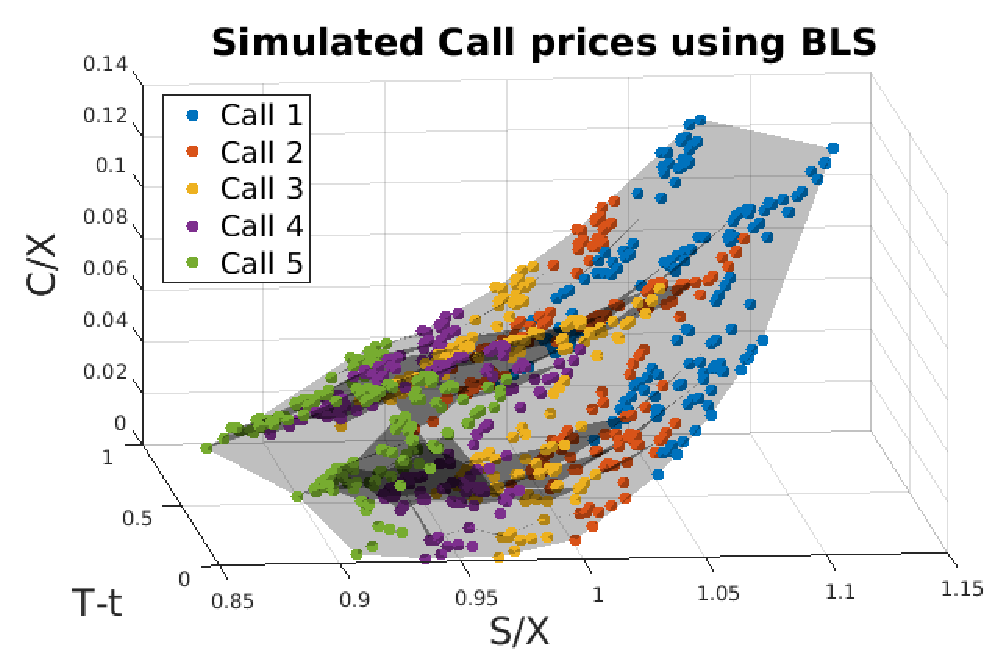
\includegraphics[scale=.6] {q1_simulated_bls.eps}
	\caption{Simulated Black-Scholes Price}
	\label{fig:q1-simulated-bls}
\end{center}
\end{figure}

Figure \ref{fig:q1-simulated-bls} is the Figure 4 in \cite{hutchinson} drawn on the validation set for all 5 call options. If the RBF network truly learnt the Black-Scholes formula from the training data, it would produce a similar result over the validation set. From Figure \ref{fig:q1-rbf-price} we can see that the RBF network produces a similar graph, as claimed in the paper. This surface was produced by using \texttt{trisurf} and \texttt{delaunay} triangulation over $S/X$, $C/X$ and $T-t$ values. The data points were plotted using \texttt{plot3}. Also, as done in Figure 5 of the paper, I plotted the validation set pricing error from the RBF network in Figure \ref{fig:q1-rbf-price}. The shape is as expected, a surface with erratic folds in the corners.\\

\begin{figure}[!h]
\begin{center}
	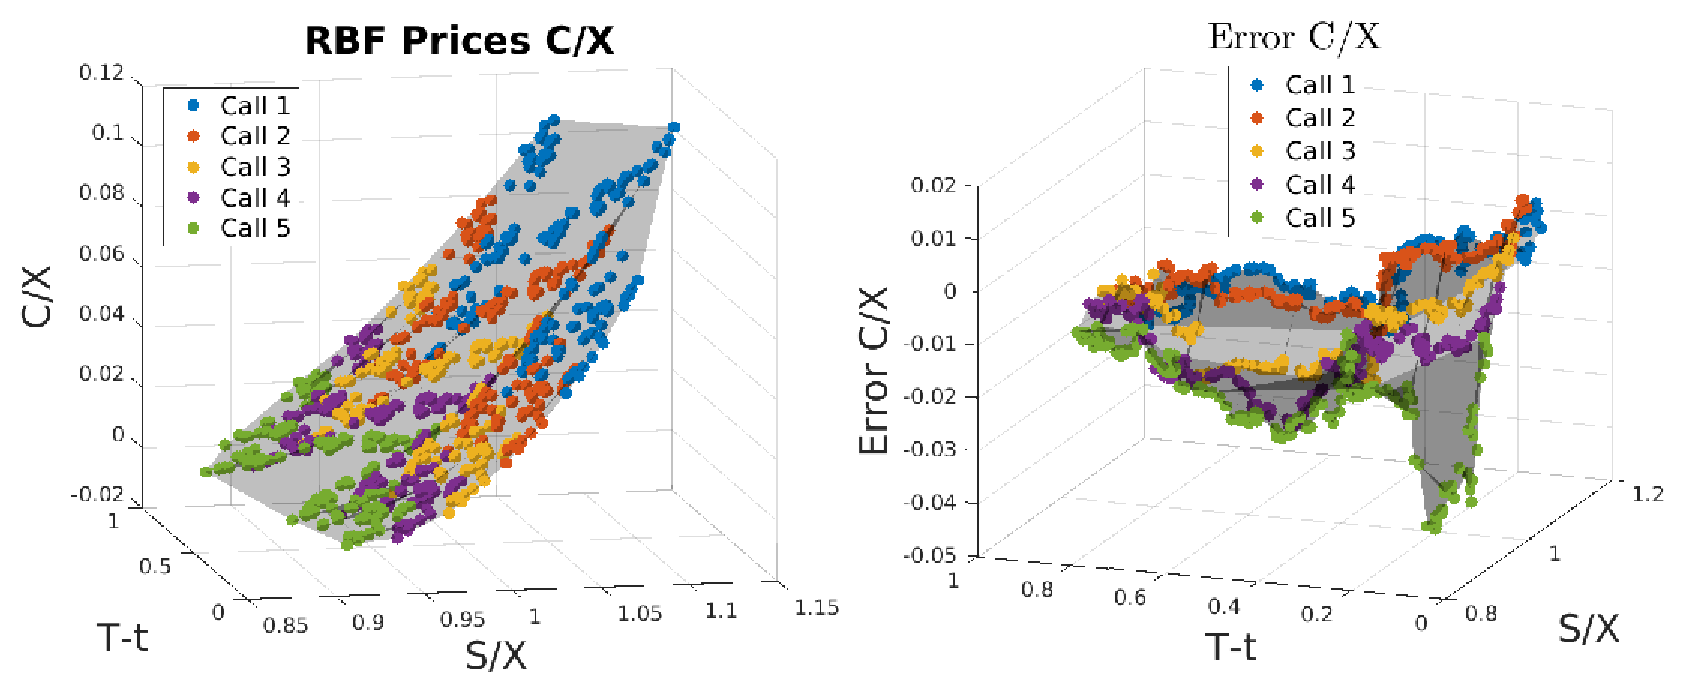
\includegraphics[scale=.6] {q1_rbf_price.eps}
	\caption{Option Price Prediction prediction from RBF Network}
	\label{fig:q1-rbf-price}
\end{center}
\end{figure}

The paper claims that the RBF network will also be able to approximate the delta values from the Black-Scholes formula. In that regard, I plotted the network deltas of the validation set in Figure \ref{fig:q1-rbf-delta}. Both the delta and delta error graphs matches the claimed graph in Figure 5 of the paper.\\

\begin{figure}[!h]
\begin{center}
	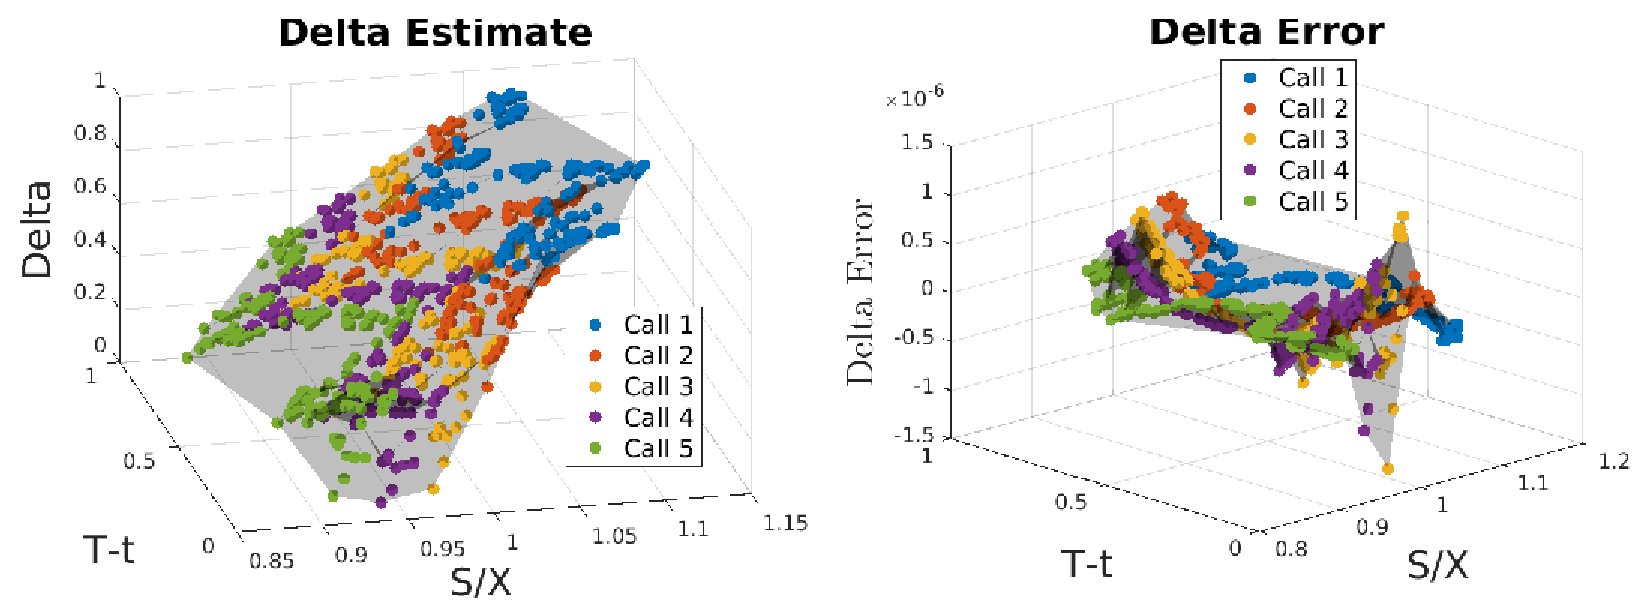
\includegraphics[scale=.6] {q1_rbf_delta.eps}
	\caption{Delta prediction from RBF Network}
	\label{fig:q1-rbf-delta}
\end{center}
\end{figure}

Finally, I plotted the boxplot of the absolute error between the actual option price, Black-Scholes model and RBF network in Figure \ref{fig:q1-bls-vs-rbf} over the validation set. It is interesting that the RBF model actually performed better than the Black-Scholes model on the validation set (although there are some outliers). This may be because the Black-Scholes model's assumptions do not hold true in real life, but the RBF model is able to cope with it. However, the actual pricing difference between these two models is in hundreths as seen in the figure.

\begin{figure}[!h]
\begin{center}
	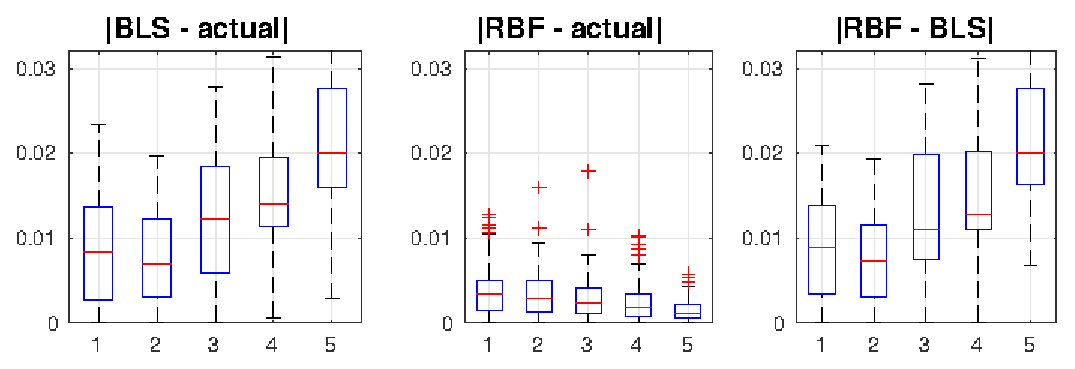
\includegraphics[scale=.65] {q1_bls_vs_rbf.eps}
	\caption{Absolute difference in pricing}
	\label{fig:q1-bls-vs-rbf}
\end{center}
\end{figure}

The experiment on the given data supports the claims in the paper. One of the non-parametric approaches to option pricing - using a trained RBF network can closely mimic the Black-Scholes formula given about 6 months worth of daily data. It also seems to have performed better than Black-Scholes in terms of matching the actual trading prices. However, it will require further investigation to assertain wheter it actually performs better, or that was a one-off scenario. Either way, it seems that a learning network gives us a much better and data derived flexibility in pricing options.

\begin{thebibliography}{9}
\bibitem{hutchinson} 
J. Hutchinson, A. Lo, and T. Poggio,
\textit{A nonparametric  approach  to  pricing  and  hedging  derivative
securities via learning networks}. 
The Journal of Finance, vol. 49, no. 3, pp. 851–889, 1994.

\end{thebibliography}

\end{document}












































